\section{Theoretical Result}\label{sec:fc}
In this section, we state three results (\Cref{th:main,th:mainconv,th:mainres}) that characterise `what is learnt in the gates of a DNN with ReLUs'.  To this end, we use the DGN setup where the gates and weights are separate. Since we are interested only in the `what?'  (and not the `how?'), we keep the gates we want to characterise \emph{fixed} in the feature network (which is a \emph{trained} DNN with ReLUs) and characterise their (i.e., gates') performance by training the value network and measuring the test performance. With reference to \Cref{prop:ntks}, since the gates fixed, it follows that $\kf=\mathbf{0}$ and we will characterise only $\kv$ which corresponds to the value network. Here, the DGN is used to study the information in gates of a \emph{trained} DNN with ReLUs. We wish to point that the gates of the DGN can also be tuned in which case $\kf\neq \mathbf{0}$, and we reserve a theoretical characterisation of $\kf$ for future work. We first begin with the following assumption that states the initial conditions of the weights of the value and the feature network weights.
\begin{assumption}\label{assmp:main}
$\Tv_0\stackrel{\text{i.i.d}}\sim\text{Bernoulli}(\frac12)$ over $\{-{\sigma},+{\sigma}\}$ and statistically independent of $\Tf_0$.
\end{assumption}
\begin{theorem}[Product of Kernels Theorem]\label{th:main} Under \Cref{assmp:main}  ($\sigma=\frac{\cscale}{\sqrt{w}}$) for FC-DGN : 
\begin{align*}
\kv_{\Tdgn_0}(x,x') \ra d\cdot \cscale^{d-1} \cdot \left(\ip{ x,x'} \cdot \Pi_{l=1}^{d-1} \frac{\ip{G_l(x),G_l(x')}}w\right), \quad\text{as}\,\, w\ra\infty 
\end{align*}
\end{theorem}
\textbf{Remarks.} From prior results \citenum{arora2019exact,cao2019generalization} it follows that the product of kernels in \Cref{th:main} characterises the training and generalisation of an infinite width DGN. We wish to add that while \Cref{th:main} is a direct `re-writing' of the Theorem~$5.1$ in \citenum{npk}, \Cref{th:main} nevertheless  explicitises the role of gates, depth and width (in a manner unknown in prior works) and forms the basis of several novel experiments in \Cref{sec:exp}. Further, while characterising the gates from a finite width network, the $w\ra\infty$ is not a restriction, because, one can `repeat' the finite width gates `infinite' number of times and apply \Cref{th:main}. Also, note that the statistical decoupling of weights and gates in \Cref{assmp:main} is unrealisable in a DNN with ReLU, however, this assumption can be trivially realised in a DGN. Note that we are interested only in the gates which we store in the feature network and are willing to reset and retrain the weights in the value network from scratch. This is justified by the experiments (see \Cref{sec:exp}) which show that such decoupling and re-training does not hurt test performance. Above all, we use the insights obtained from \Cref{th:main} as a indicator of the trends that we can expect when we experiment with finite width networks. We now discuss the key insights.

\textbf{Key Insights.} \Cref{th:main} suggets the following decomposition: (i) the feature network is responsible for the gates, i.e. the features $G_l(x)$ and (ii) the value network implements the product of kernels by laying out the gates as masks depth-wise, and connecting them in the structure of a DNN. For instance, if we were to concatenate the gating features as $\varphi(x)=(G_l(x),l=1,\ldots,d-1)\in\{0,1\}^{(d-1)w}$, it would have only resulted in the kernel $\ip{\varphi(x),\varphi(x')}=\sum_{l=1}^{d-1}\frac{\ip{G_l(x),G_l(x')}}w$, i.e., a \emph{sum  (not product)} of kernels. Thus, at the heart is the \emph{\textbf{correlation of the gates}} given by the \emph{\textbf{base kernel}} $\frac{\ip{G_l(x),G_l(x')}}w$, where the role of width is averaging (division by $w$). 

\textbf{Convolutions with pooling.} Let the circular rotation of vector $x\in\R^{\din}$ by `$r$' co-ordinates be defined as $rot(x,r)(i)=x(i+ r)$, if $i+r \leq \din$ and $rot(x,r)(i)=x(i+ r-din)$ if $i+r > \din$. Using circular convolutions with pooling results in a rotationally invariant kernel \Cref{th:mainconv}. The architecture and the notations for the network with convolutions is presented in the Appendix.
\begin{comment}
 We extend the dual view to neural network with $\dc$ convolutional layers ($l=1,\ldots,\dc$), followed by a \emph{global-average/max-pooling} layer ($l=\dc+1$) and $\dfc$ ($l=\dc+2,\ldots,\dc+\dfc+1$) fully connected  layers (see Appendix for notation). The convolutional window size is $\wconv<\din$, the number of filters per convolutional layer as well as the width of the fully connected layers is $w$. The main steps are (i) treating pooling layers like gates/masks, (ii) bundling together the paths that share the same path value (due to weight sharing in convolutions) and (iii) re-defining the NPF and NPV for these bundles. The important consequence of weight sharing (due to convolutions and pooling) is that the NPK becomes rotationally invariant resulting in \Cref{th:mainconv}.
\end{comment}
\begin{theorem}[Rotationally Invariant Kernel Theorem]\label{th:mainconv} Under \Cref{assmp:main}, for  a suitable $\bcnn$:
\begin{align*}
&\kv_{\Tdgn_0}&\ra&\quad \frac{\bcnn}{{\din}^2} \cdot \sum_{r=0}^{\din-1} \ip{x,rot(x',r)}_{\Lambda(\cdot, x,rot(x',r))},\,\, \text{as}\,\,  w\ra\infty\,\text{(for global-average-pooling)}, \\
&\kv_{\Tdgn_0}&\ra& \quad{\bcnn} \cdot \sum_{r=0}^{\din-1} \ip{x,rot(x',r)}_{\Lambda(\cdot, x,rot(x',r))},\,\, \text{as}\,\,  w\ra\infty\,\text{(for global-max-pooling)}
\end{align*}
\end{theorem}
\textbf{Remark.}  $\Lambda(i,x,x')$ counts the number of paths starting from input node $i$ that are active for both $x$ and $x'$. The summation can be expanded as $\sum_{r=0}^{\din-1} \ip{x,rot(x',r)}_{\Lambda(\cdot, x,rot(x',r))}=\sum_{r=0}^{\din-1} \left(\sum_{i=1}^{\din} x(i) rot(x',r)(i)\Lambda(i,x,x')\right)$, where the inner $\Sigma$ is the inner product between $x$ and $rot(x',r)$ weighted by $\Lambda$ and the outer $\Sigma$ covers all possible rotations.

\textbf{Residual Networks with Skip connections.} We consider a ResNet with `$(b+2)$' blocks and `$b$' skip connections between the blocks (left of \Cref{fig:resnet}). Each block is a fully connected (FC) DNN of depth `$\dblock$' and width `$w$'. There are combinatorially many sub-FC-DNNs within this ResNet (see \Cref{def:subfcdnn} and right of \Cref{fig:resnet}).
\FloatBarrier
\begin{figure}[h]
\begin{minipage}{0.5\columnwidth}
\resizebox{\columnwidth}{!}{
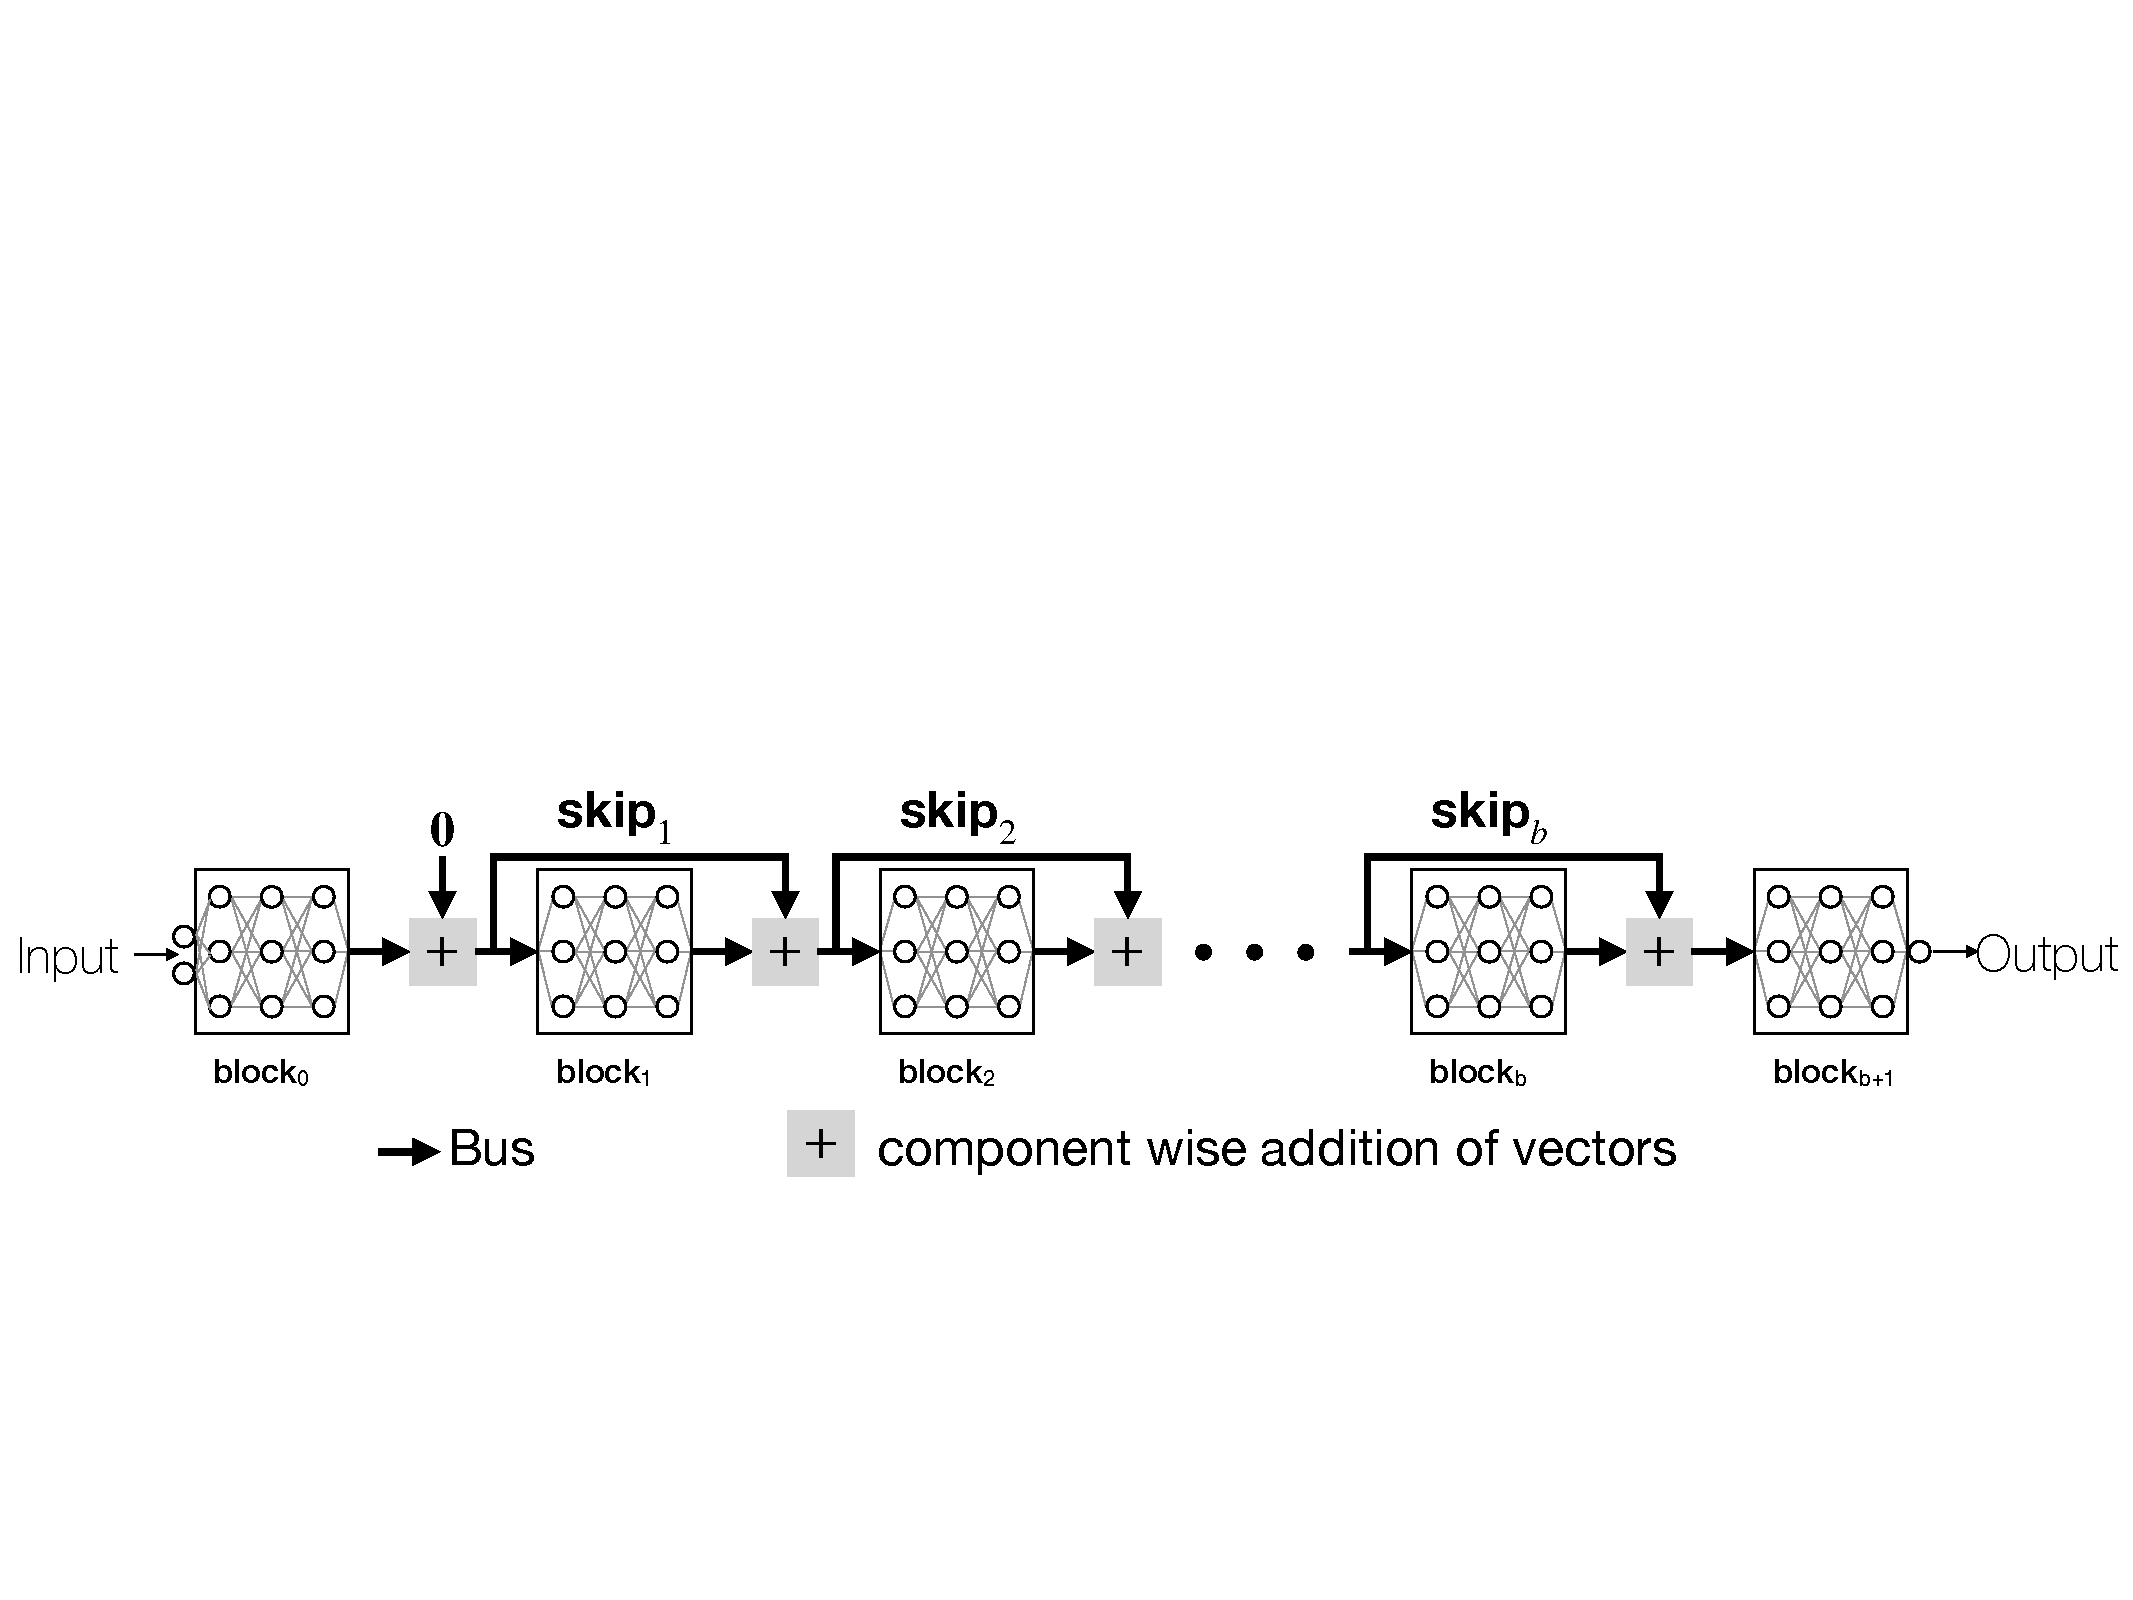
\includegraphics[scale=0.5]{figs/resnet.pdf}
}
\end{minipage}
\begin{minipage}{0.5\columnwidth}
\resizebox{\columnwidth}{!}{
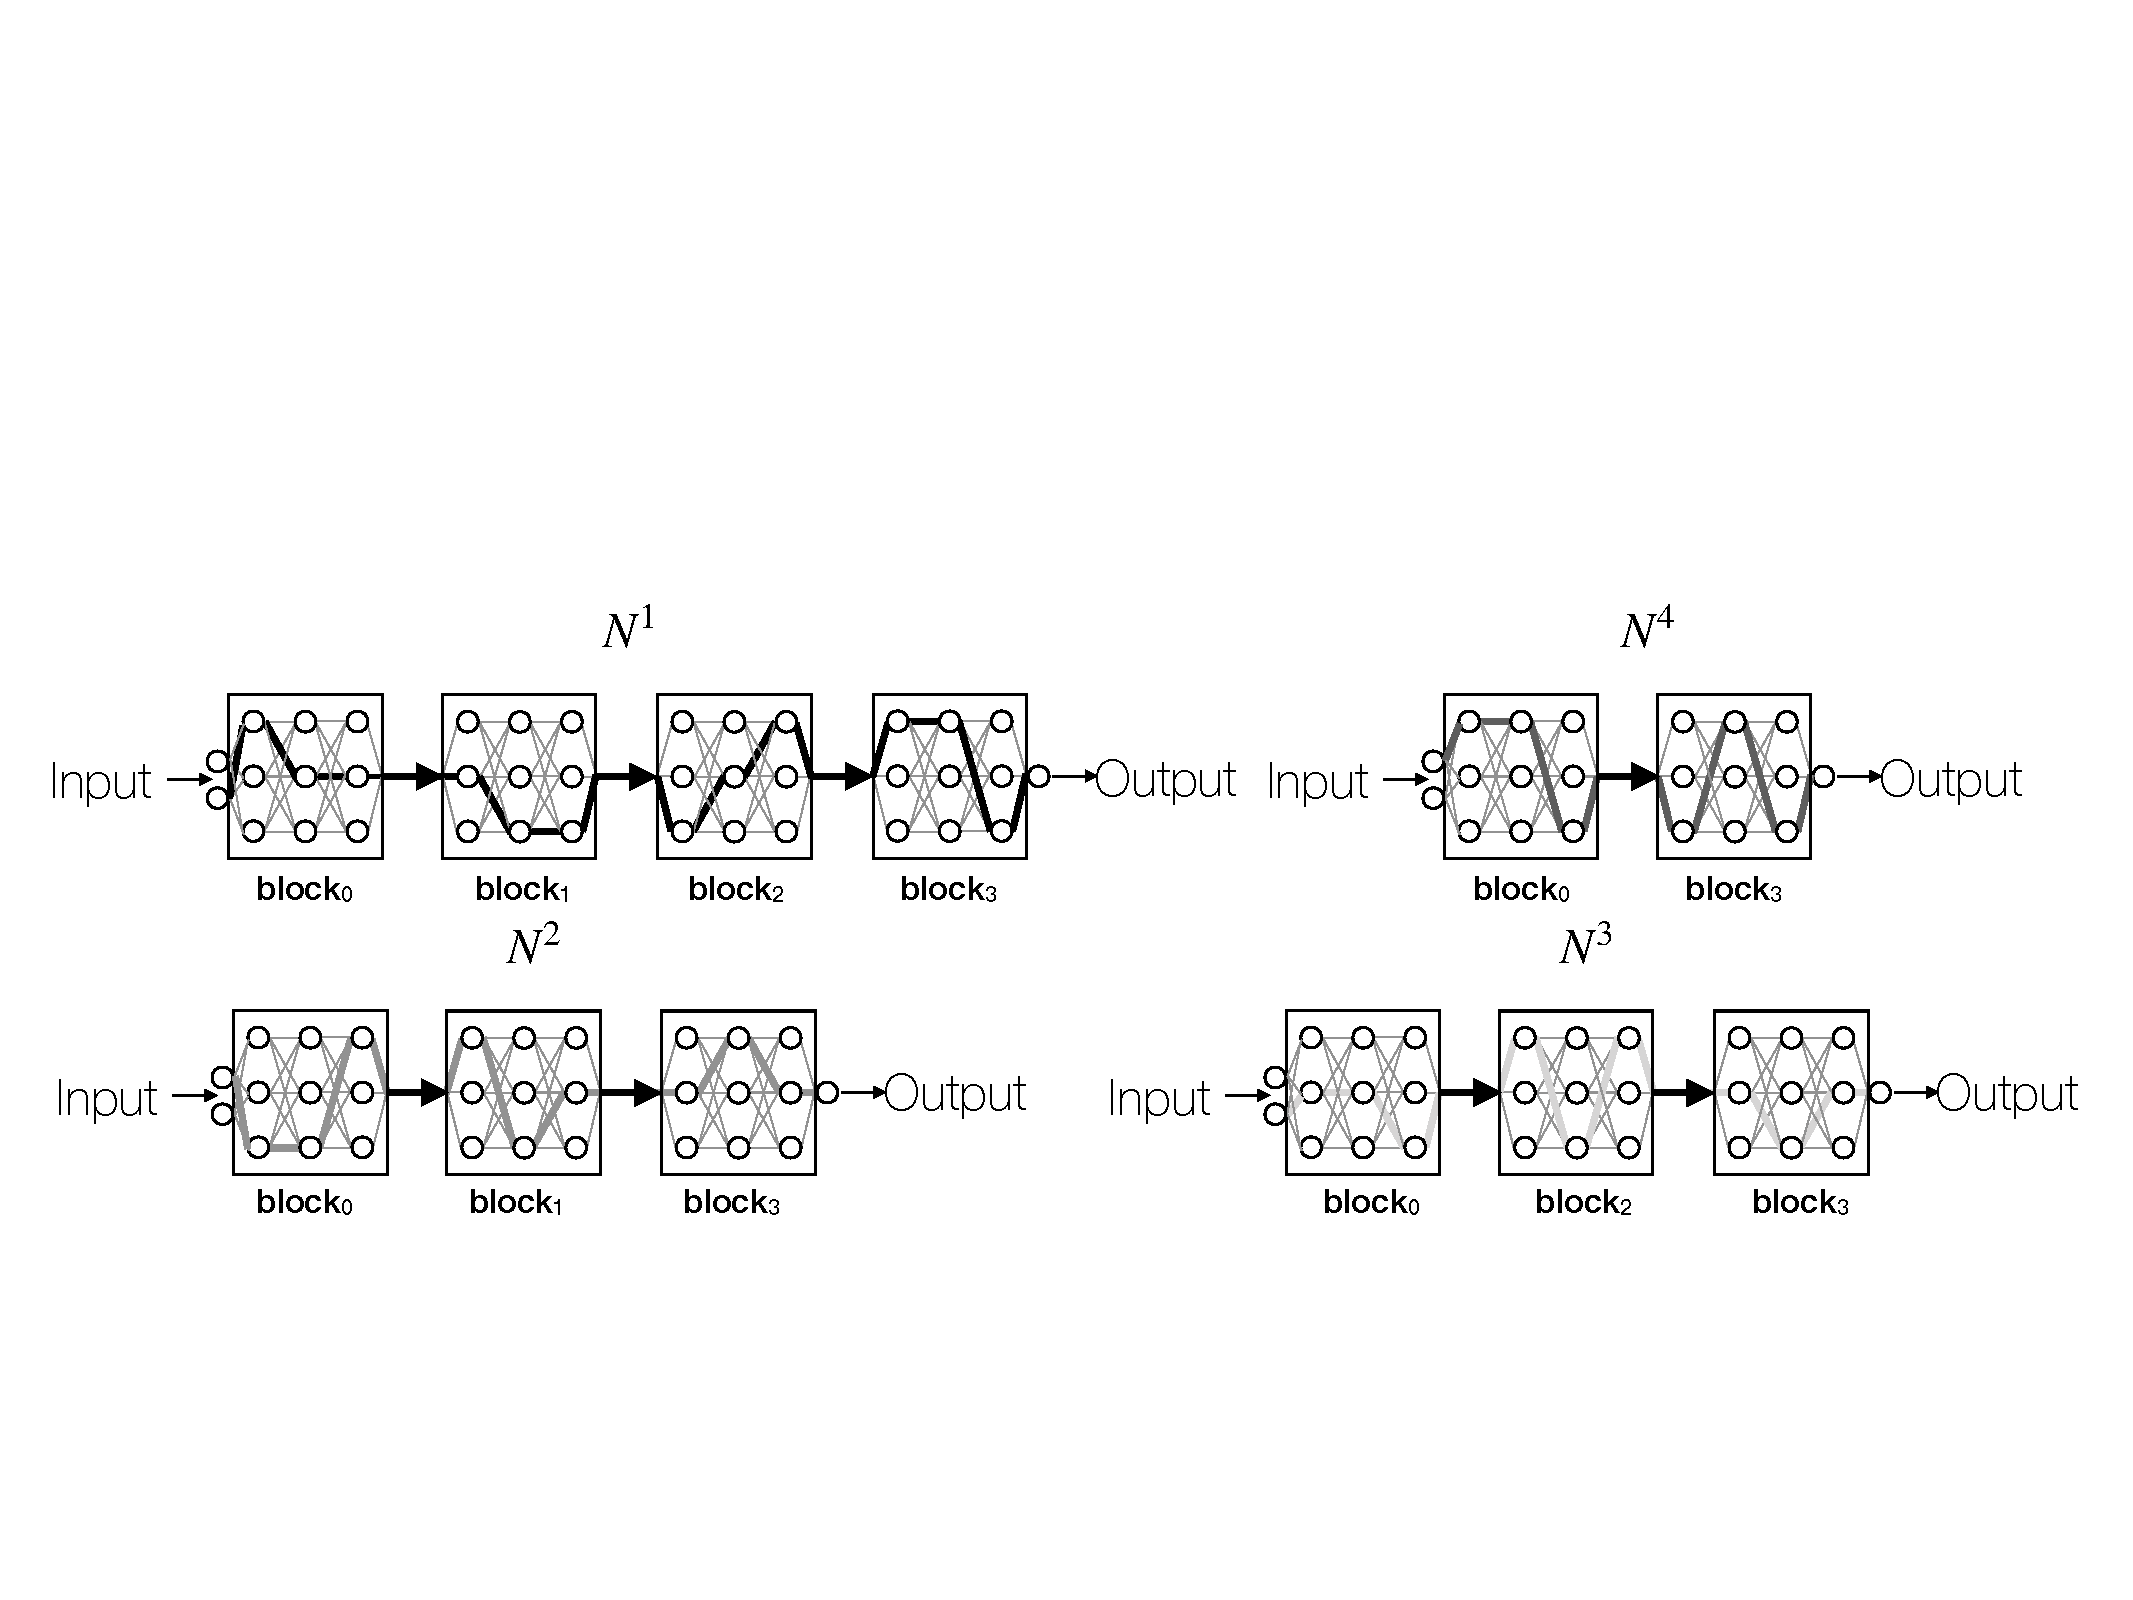
\includegraphics[scale=0.5]{figs/blocks.pdf}
}
\end{minipage}
\caption{\small{On the left is the ResNet with $b$ skip connections and $(b+2)$ blocks. On the right are the sub-FC networks $N^1$ obtained by skipping no blocks, $N^2$ and $N^4$ obtained by skipping block $1$ and $2$ respectively, and $N^3$ obtained by skipping both blocks $1$ and $2$.}}
\label{fig:resnet}
\end{figure}

\begin{definition}\label{def:subfcdnn}[Sub FC-DNNs]
Let $2^{[b]}$ denote the power set of $[b]$ and let $\J\in 2^{[b]}$ denote any subset of $[b]$. Define the`$\J^{th}$' sub-FC-DNN of the ResNet to be the fully connected network obtained by (i) ignoring/removing the skip connections $\text{skip}_j,\forall j\in \J$  and (ii) ignoring $\text{block}_{j},\forall j\notin \J$ (see \Cref{fig:resnet}).
\end{definition}
\begin{theorem}[Sum of Product of Kernels Theorem]\label{th:mainres} Let $H^{\J}_{\Tf_0}$ be the NPK of the $\J^{th}$ sub-FC-DNN, and $\bfc^{\J}$ be the associated constant. Under \Cref{assmp:main}, we have:
\begin{align*}
\kv_{\Tdgn_0}\ra \sum_{\J\in 2^{[b]}}  \bfc^{\J} H^{\J}_{\Tf_0}, \,\, \text{as}\,\,  w\ra\infty
\end{align*}
\end{theorem}
\textbf{Note.} The sub-FC-DNNs we refer to in \Cref{th:mainres} belong to (or are parts of) the feature network from which the gates are obtained. 
%\end{comment}